\documentclass{article}

\usepackage[english]{babel}
\usepackage[letterpaper,top=2cm,bottom=2cm,left=3cm,right=3cm,marginparwidth=1.75cm]{geometry}
\usepackage{amsmath}
\usepackage{graphicx}
\usepackage{float}
\usepackage{subcaption}
\usepackage[colorlinks=true, allcolors=blue]{hyperref}


\usepackage[
backend=biber,
style=alphabetic,
sorting=ynt
]{biblatex}
\addbibresource{SPCSimLib.bib}

\title{Determining the accuracy of FreeRunning mode versus Parallel mode as well as the accuracy of Equi-Width Histograms versus Equi-Depth Histograms under variable Attenuation using SPCSimLib \cite{spc}}
\author{Elliott VanOrman, intern with the Institute for Computing in Research}

\begin{document}
\maketitle

\begin{abstract}
This paper compares the error in results of a Single Photon Camera (SPC) when using Equi-Width Histograms (EWH) versus Equi-Depth Histograms (EDH), parallel versus asynchronous data collection, and 1.5 FWHM versus 5.0 FWHM laser pulses
Data was collected using the python library SPCSimLib, specifically by simulating a single SPC pixel, and measuring the error each method produced.
Our analysis showed using Equi-Width Histograms, asynchronous data collection, or 1.5 FWHM pulses creates pictures matching reality more closely than those created using Equi-Depth Histograms, parallel data collection, or 5.0 FWHM pulses, to a statistically significant level.
from this, we concluded that using Equi-Width Histograms, Asynchronous data collection and 1.5 FWHM pulses produces more accurate results than using Equi-Depth Histograms, Parallel data collection, and 5.0 FWHM pulses.
\end{abstract}

\section*{Introduction}

Single Photon Cameras, or 'SPC's for short, are cameras that function similarly to LIDAR, in that they produce 3D photographs by measuring the time it takes for light to travel to a point and bounce back. Unlike LIDAR however, SPCs use individual photons instead of lasers. \cite{ingle} \cite{sadekar}

When a picture is taken, the SPC begins sending out pulses of photons towards the thing it is taking a picture of. When these photons are reflected back onto the detector, it records the timestamp. We can then calculate the distance away from our camera using the formula \[D=C*T*\frac{1}{2}\] where $D$ is distance, $T$ is the time it took photons to reflect back to the detector and $C$ is the speed of light. \cite{sadekar}

There are almost always ambient photon levels, however, meaning that while timestamps do cluster around the 'true' time it took photons to reflect back, there are a certain number of 'noise' timestamps due to background illumination. There are multiple methods to determine when the true center of the pulse (called the 'peak') is located. After the 'peak' is located, it is used as $T$ in the previously shown formula \cite{sadekar}.

Taking an accurate picture, collecting data accurately, and sorting the noise from the real data is quite complicated however, and there are several factors to consider. Namely:
\begin{itemize}
\item The kind of histogram used to locate the peak.
\item Whether collectors collect data asynchronously or in parallel.
\item How long the laser fires.
\end{itemize}

There are two types of histograms to use when finding the peak: \cite{sadekar}
\begin{itemize}
\item Equi-Width Histograms, histograms with buckets of equal width but variable depth. For EWHs, The 'peak' bucket is the bucket with most detections.
\item Equi-Depth Histograms, histograms with buckets of variable width but equal depth. For EDHs, the 'peak' bucket is the bucket of the shortest width.
\end{itemize}
In both cases, The center of the 'peak' bucket is recorded as the 'peak' of the pulse.

Before explaining asynchronous data collection the difference between asynchronous mode and parallel mode, it would be helpful to gain a working understanding of deadtime.
Due to the physical limitations of SPC cameras photon readings over time do not always match reality. when a detector is hit by a photon, it takes a certain amount of time for said detector to log a timestamp. While this time is in progress, the detector cannot record new hits. In other words, a detector cannot start recording a new timestamp until it has finished recording the first, meaning photons that hit the detector during that recording time go undetected. This time is usually around 75ns, and is refered to as 'deadtime'. \cite{sadekar}

There are two modes in which one collects data: \cite{sadekar}
\begin{itemize}
\item Parallel (or, Not FreeRunning) Mode. In Parallel mode, detectors are reset at the beginning of each pulse, prematurely ending their deadtime. due to earlier photons blocking out later photons however, this often results in right-skewed timestamp data.
\item Asynchronous (or, FreeRunning) Mode. In Asynchronous mode, detectors are allowed to run until their deadtime elapses in full. This takes in less photons, but produces more uniform data.
\end{itemize}

Then there is how long the laser fires, measured by taking the Full Width at Half Maximum of the parabola measuring the intensity of the laser:
\begin{itemize}
\item FWHM, unlike histograms and modes, is a continous measurement of how long each laser pulse fires.
\item FWHM, or Full Width at Half Maximum, refers to the length of the curve of intensity of the laser when it fires. It can also affect the error of the laser, as the increaed length of the laser would also increase the width of the 'peak' of the pulse.
\end{itemize}

Unfortunately, due to right-skewed data, it often becomes necesary to filter out a certain percent of incoming photons. this filtering is called 'attenuation', \cite{ingle} and while it may reduce the overal number of photons hitting an SPC, the fact that any one datapoint blocks other datapoints from being recorded for a period of time causes it to actually increase the amount of photons not blocked by early recordings, producing less skewed  data and increasing accuracy.  \cite{sadekar}

As we have explained, there are many methods that can be used to receive and interpret data from SPCs, but it has not yet been determined which produces the most accurate results. It was hypothesized that:
\begin{itemize}
  \item Equi-depth histograms with 16 buckets would produce more accurate results than Equi-Width histograms with 1000 buckets
  \item Asynchronous (non-FreeRunning) mode would produce more accurate results than Parallel (FreeRunning)
  \item 1.5 FWHM lasers would produce the same amount of error as 5.0 FWHM lasers.
\end{itemize}
  
\section*{Method}
In order to determine what produced the most accurate results, we used the Python library SPCSimLib \cite{spc} to simulate a pixel of an SPC. To find error, we simulated taking a picture with an SPC. We then subtracted the 'true distance' (The distance from the camera the surface being photographed was in the simulation) from the 'estimated distance' (The distance from the camera of the same surface that the SPC in the simulation estimated). After taking this difference, we normalized it by dividing it by the scale of the distance. This normalized difference is what we refer to when we say 'error'. To miminize the error in our error measurements caused by fluctuations in our error measurements, we did this ten times and took the average. After taking error measurements for every 101 percentage values of attenuation running from 0\% to 100\%, we put this data into a 'dataset', labeled it with the settings the SPC used while simulations were being taken, then saved said dataset to \href{https://github.com/yggaraxyg/SPCErrorLowerer/tree/master/RunData/runDataUsedInInitialProject}{this folder in our project's github repo}. We then changed the settings, and repeated the process in order get the data we analyzed. We then graphed this data in the formats shown below for ease of understanding saving them to \href{https://github.com/yggaraxyg/SPCErrorLowerer/tree/master/Graphs}{this folder in our project's github repo}.

\begin{figure}[H]
\centering
\begin{subfigure}[b]{1\textwidth}
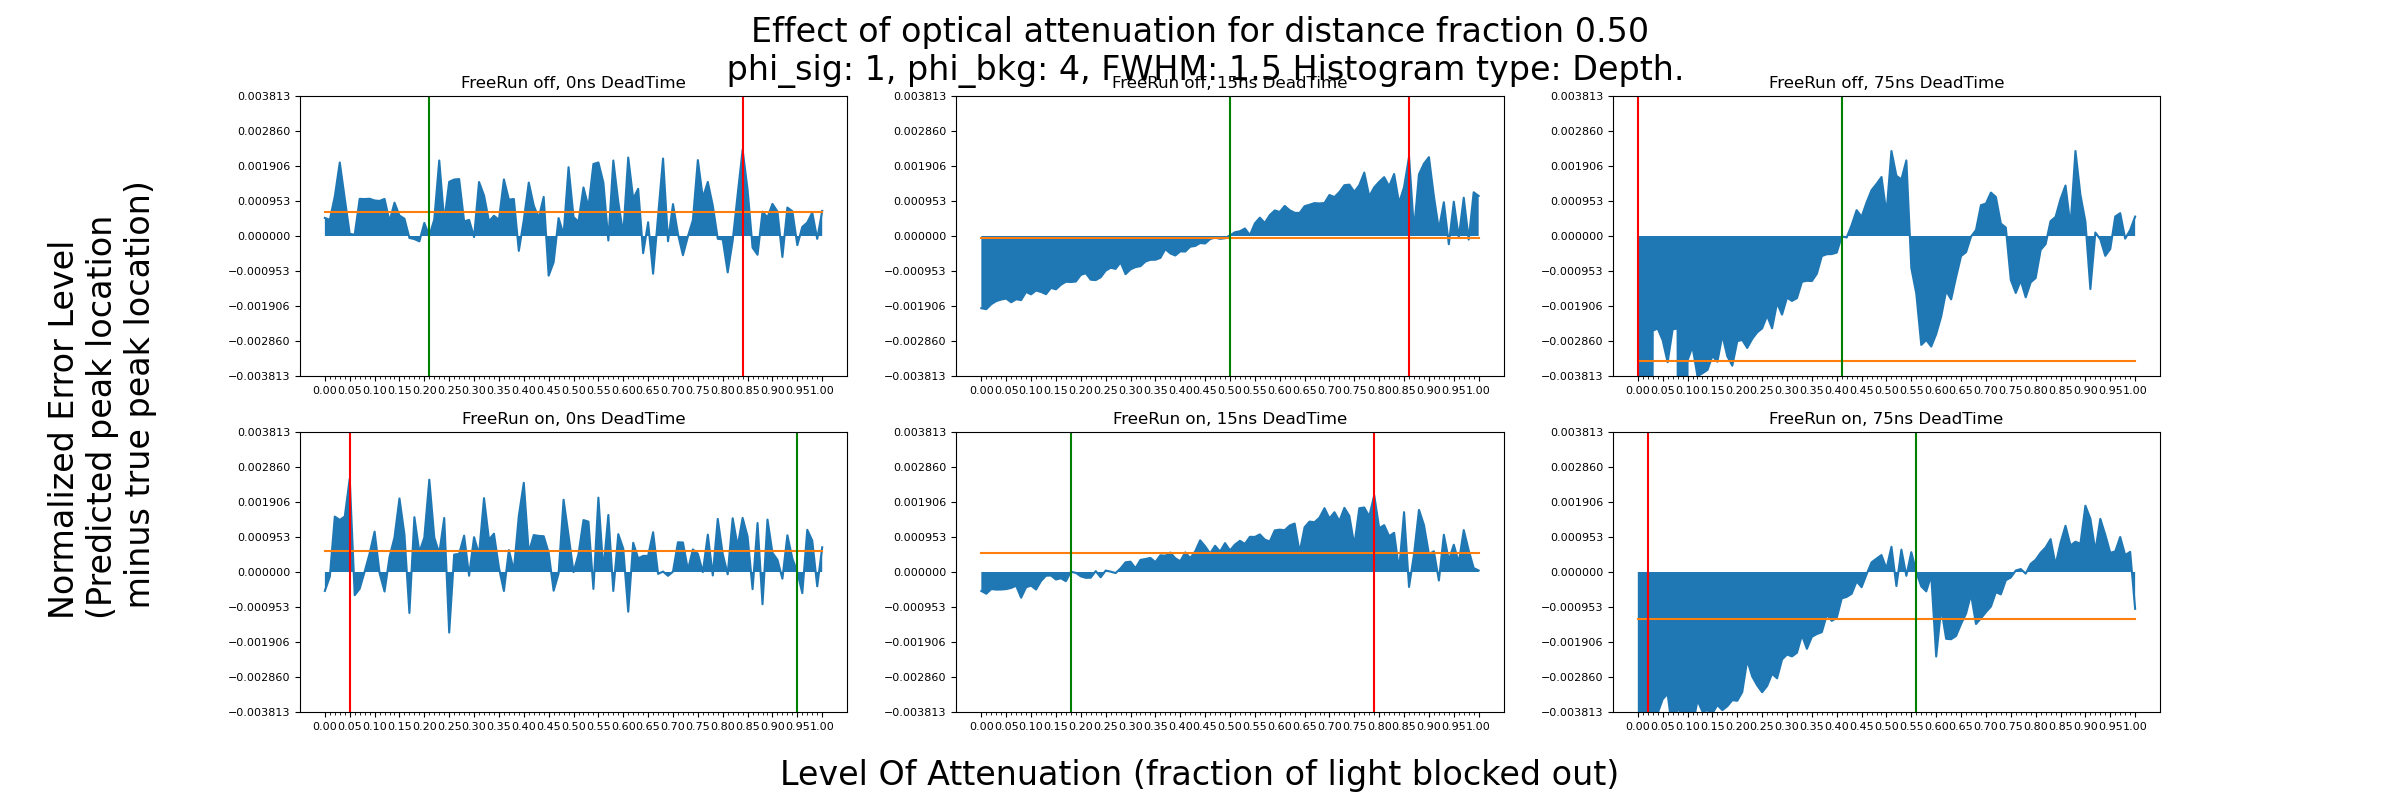
\includegraphics[width=1\linewidth]{SharedyExample.png}
\label{fig:Ng1}
\end{subfigure}
\begin{subfigure}[b]{1\textwidth}
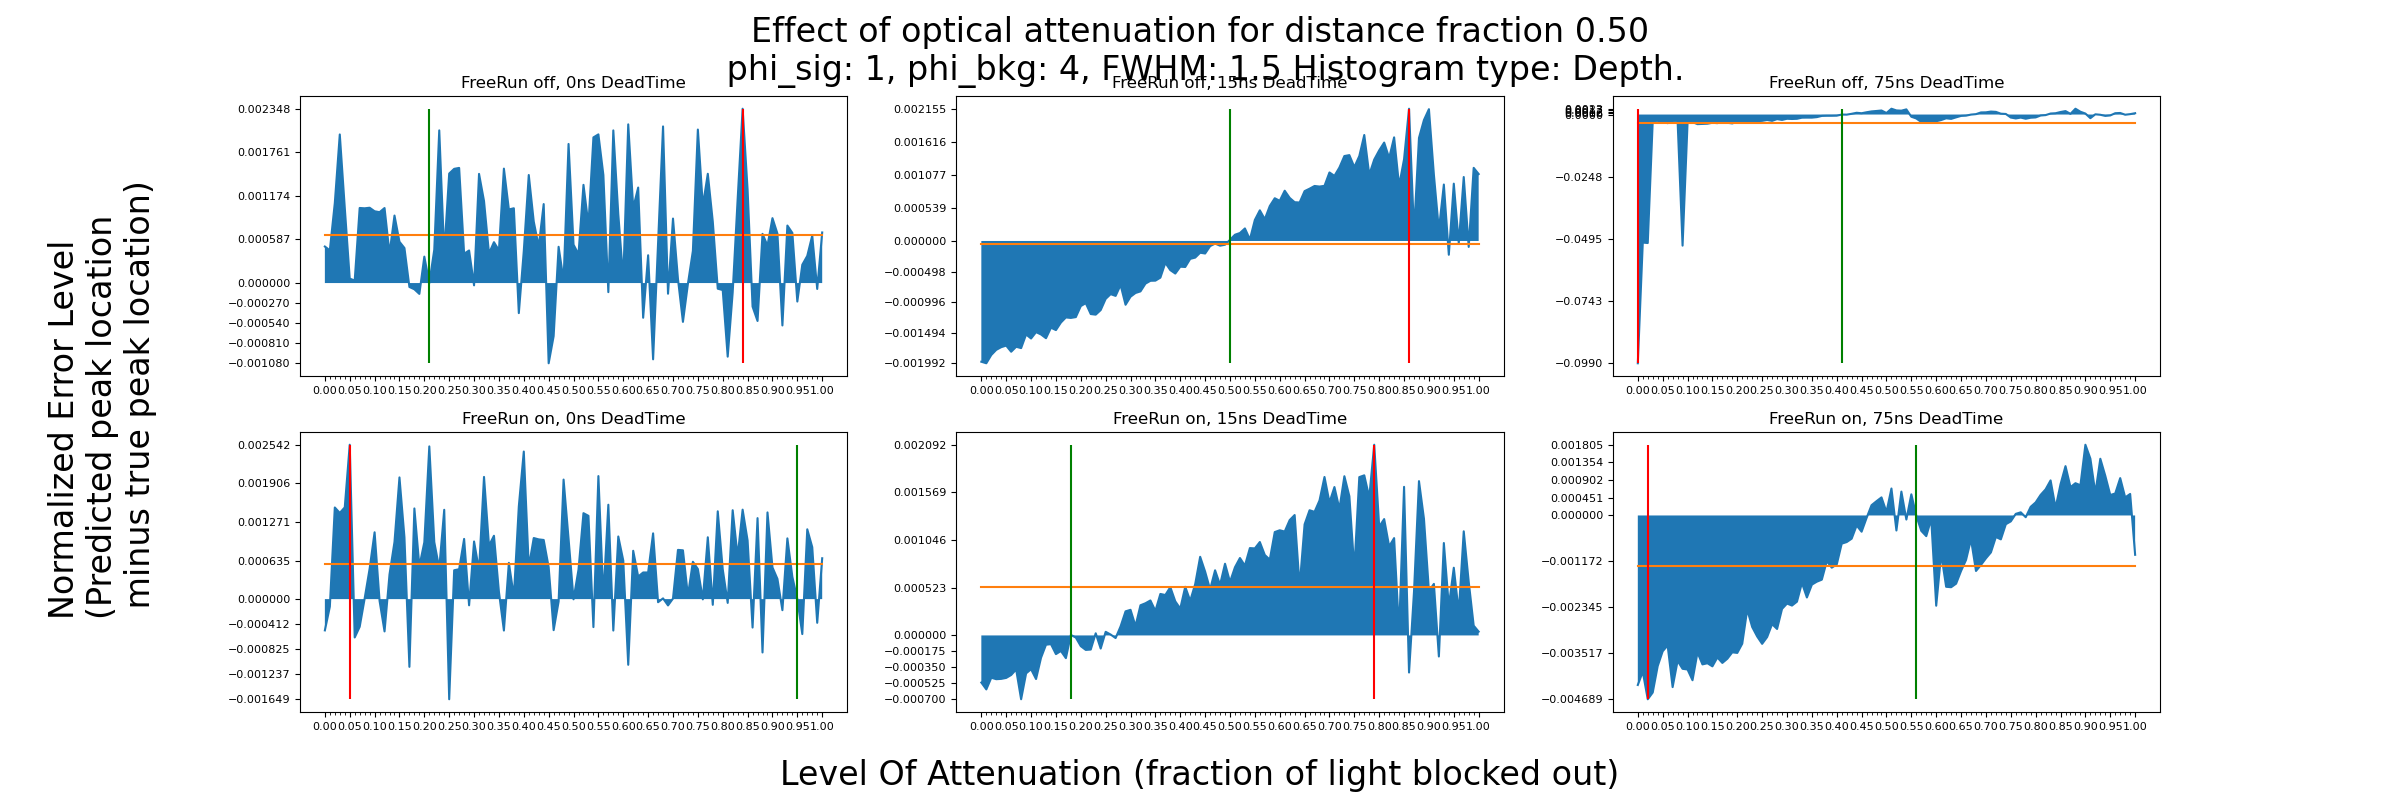
\includegraphics[width=1\linewidth]{ZoomedyExample.png}
\label{fig:Ng2}
\end{subfigure}
\caption{\label{fig:Data}The top graph and the bottom graph present the same data in two different formats. The top graph represents error on the same scale across all graphs, while the bottom represents each dataset with it's own scale. Blue represents normalized error. Orange is the mean error for all attenuation values. Red is the attenuation value which produced the least accurate result. Green is the attenuation value which produced the most accurate result.}

\end{figure}

In addition, we ran statistical analysis on the data to check our hypotheses. To do this, we put all our data in two large datasets for every hyposis, one for each differing state in the hypothesis each state is relevant to. For every hypothesis, we marked the first dataset $d_{1}$ and the second dataset $d_{2}$. We then performed a paired t-test on the data, where each observation's partner was an observation taken under circumstances identical to the first's except for the variable being tested. 

\section*{Results}
Using Paired t-tests, we found the following $T$s and P-Values for the following hypotheses:
\begin{itemize}
  \item $\mu_{EDH}=\mu_{EWH}$: $T=14.59122, df = 96959$ 
  \begin{itemize}
    \item $\mu_{EDH}>\mu_{EWH}$: $p=1.79689\times10^{-48}$
    \item $\mu_{EDH}\neq\mu_{EWH}$: $p=3.59378\times10^{-48}$
    \item $\mu_{EDH}<\mu_{EWH}$: $p=1.0$
  \end{itemize}  
  \item $\mu_{F}=\mu_{nF}$: $T=-31.63417, df = 96959$
  \begin{itemize}
    \item $\mu_{F}>\mu_{nF}$: $p=1.0$
    \item $\mu_{F}\neq\mu_{nF}$: $p=1.63522\times10^{-218}$
    \item $\mu_{F}<\mu_{nF}$: $p=8.17611\times10^{-219}$
  \end{itemize}
  \item $\mu_{1.5}=\mu_{5.0}$: $T=-55.67372, df = 96959$
  \begin{itemize}
    \item $\mu_{1.5}>\mu_{5.0}$: $p=1.0$
    \item $\mu_{1.5}\neq\mu_{5.0}$: $p=0$
    \item $\mu_{1.5}<\mu_{5.0}$: $p=0$
  \end{itemize}
\end{itemize}

All alternatve hypotheses with p-values less than 0.01 accepted. Graphs showing examples of the accepted hypotheses are as follows:

\begin{figure}[H]
\centering
\begin{subfigure}[b]{1\textwidth}
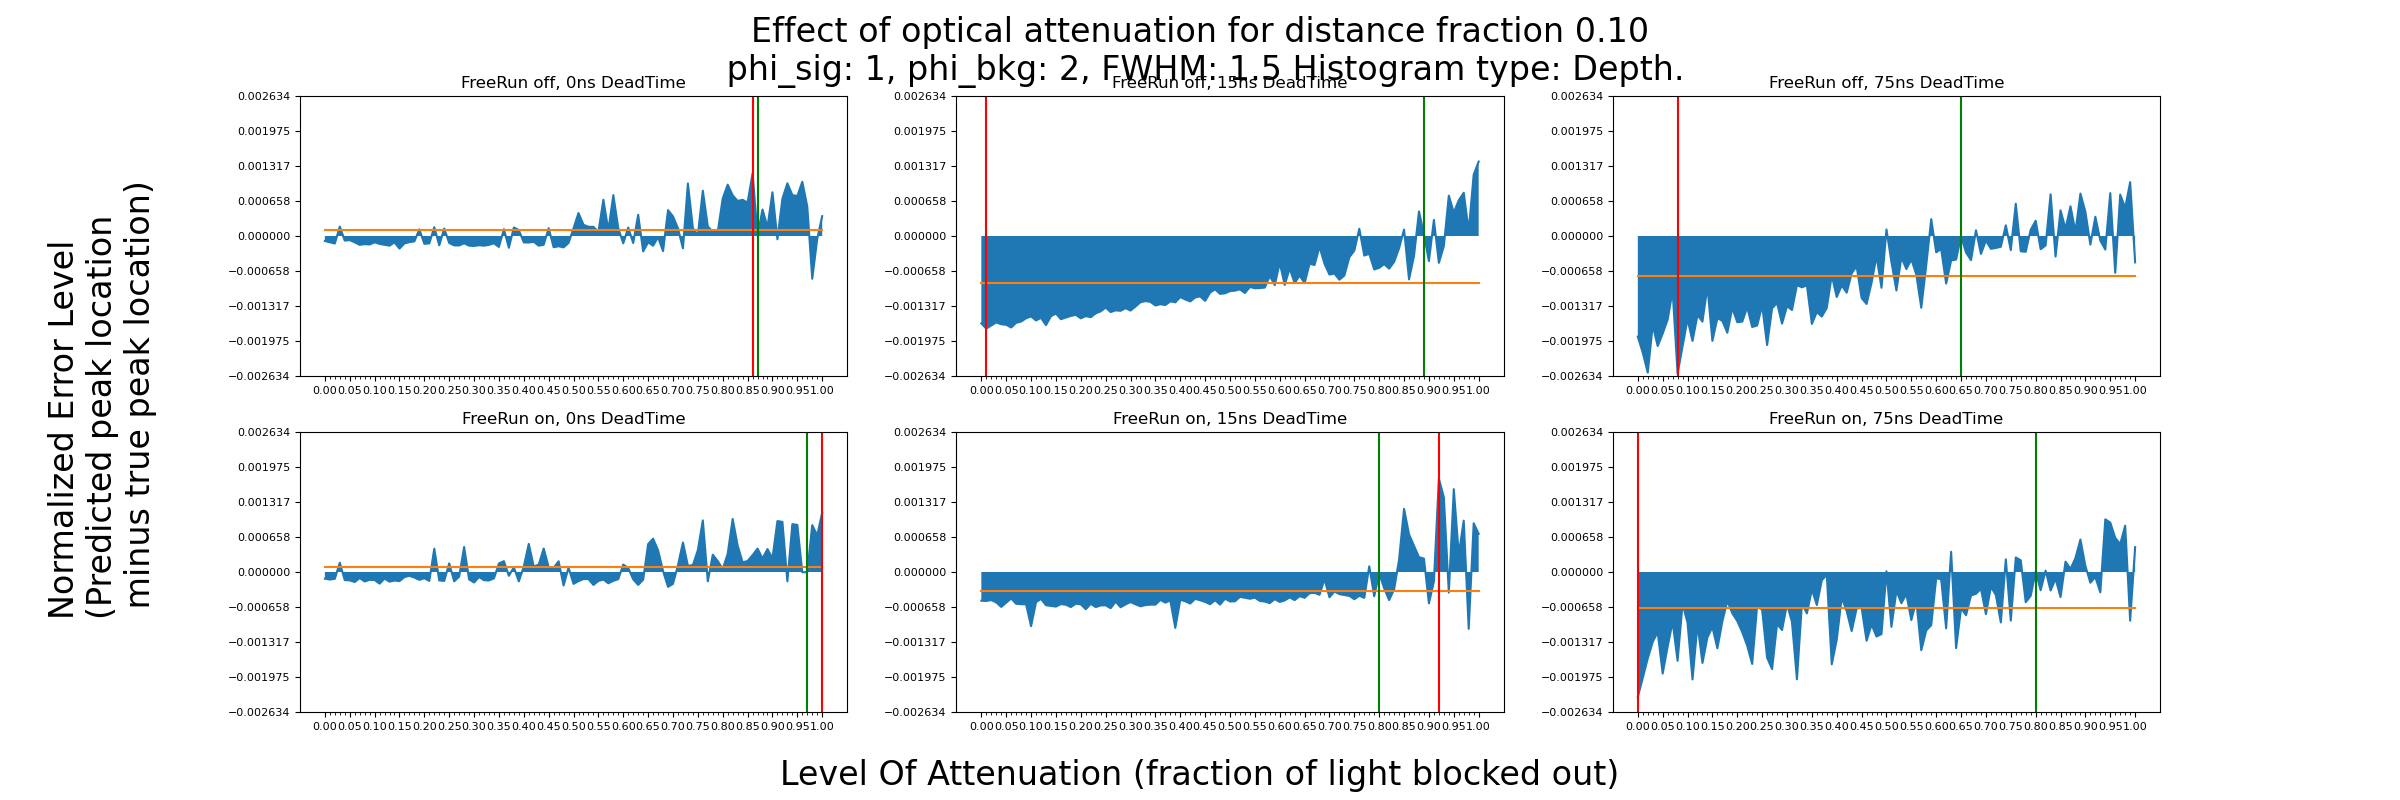
\includegraphics[width=1\linewidth]{depthExample.png}
\label{fig:Depth Example}
\end{subfigure}
\begin{subfigure}[b]{1\textwidth}
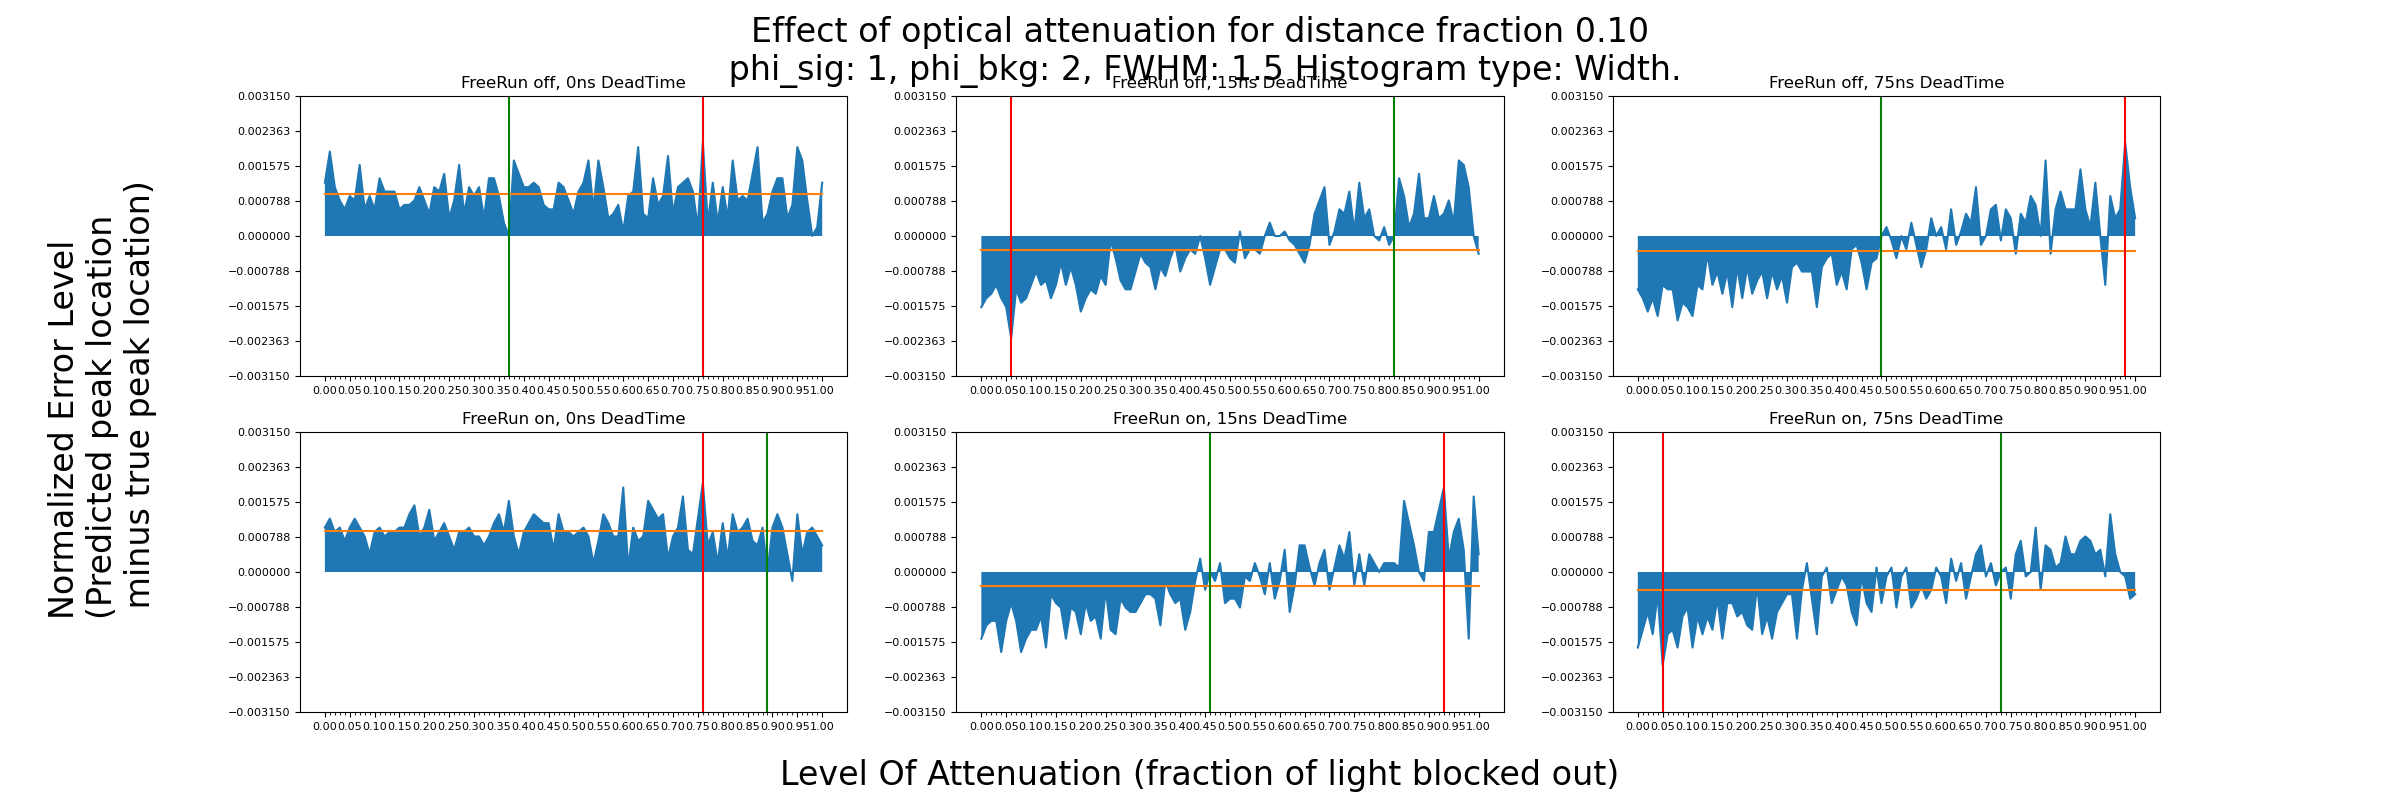
\includegraphics[width=1\linewidth]{widthExample.png}
\label{fig:Width Example}
\end{subfigure}
\caption{\label{fig:histogramComparison}EDH vs EWH}
\end{figure}

\begin{figure}[H]
\centering
\begin{subfigure}[b]{1\textwidth}
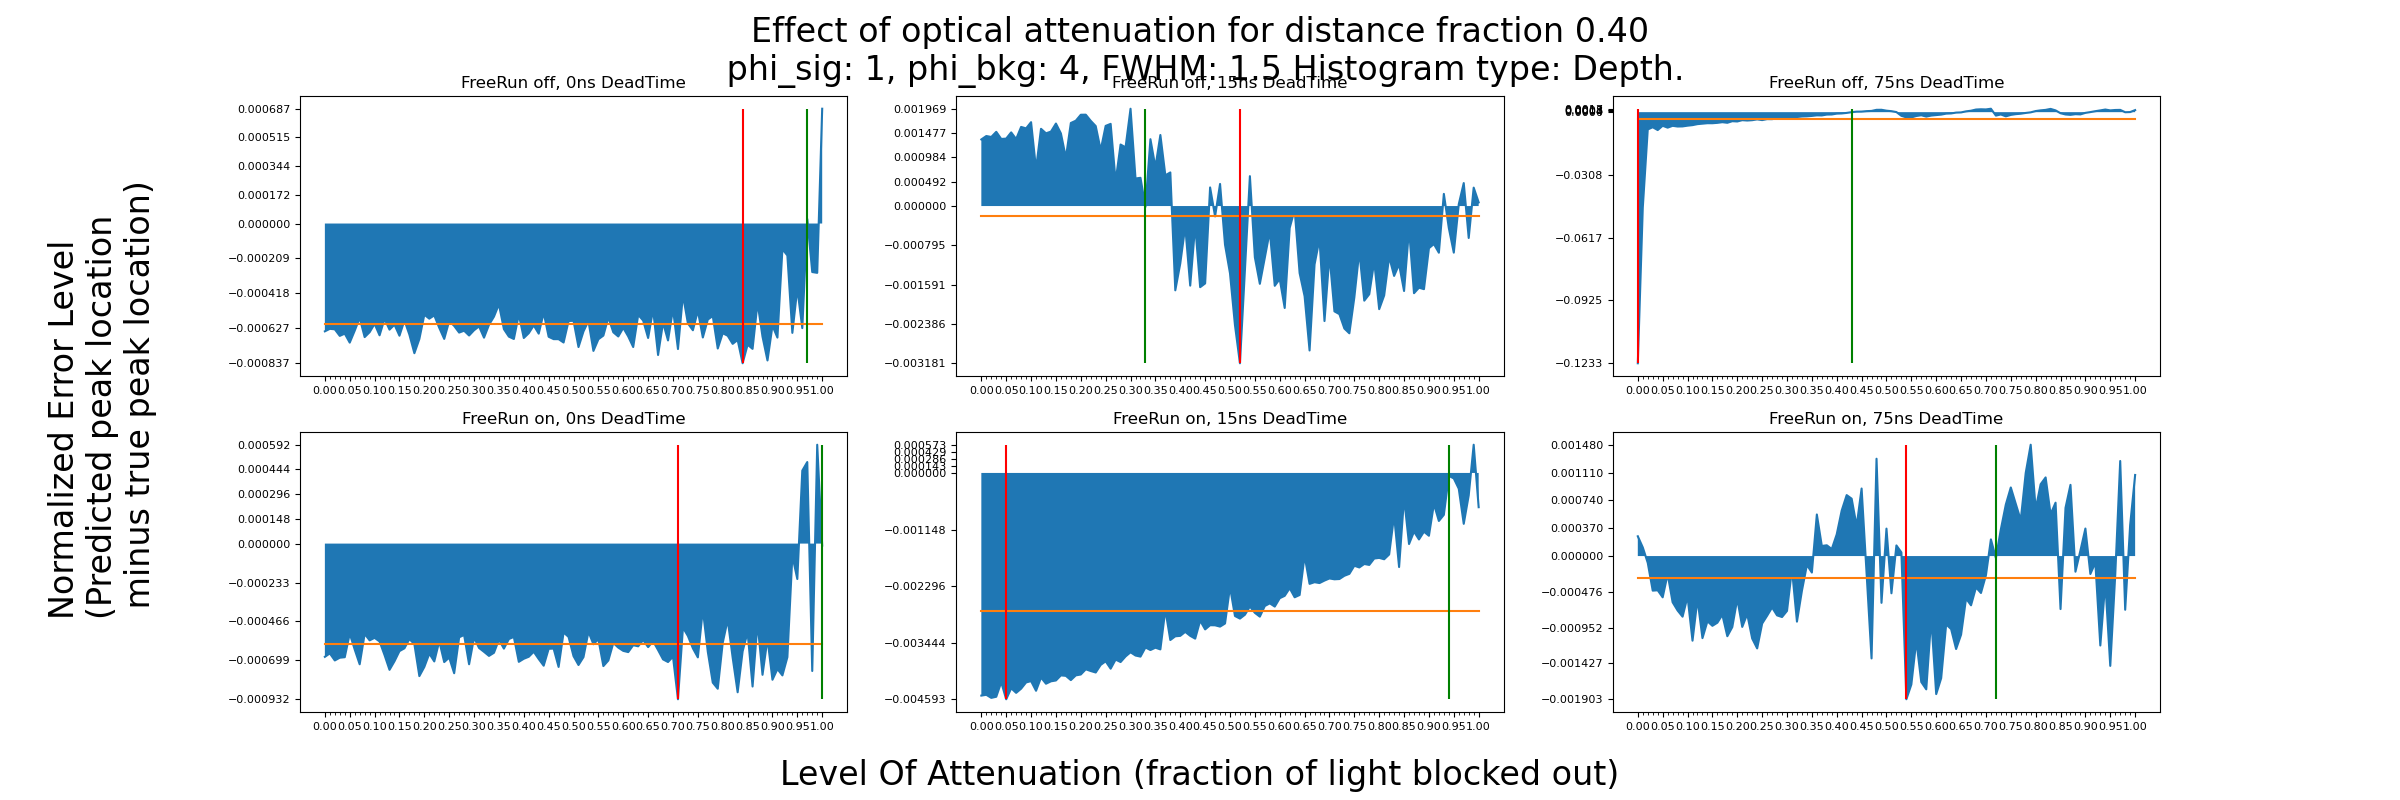
\includegraphics[width=1\linewidth]{zoomedFreeExample.png}
\label{fig:zoomedExample}
\end{subfigure}
\begin{subfigure}[b]{1\textwidth}
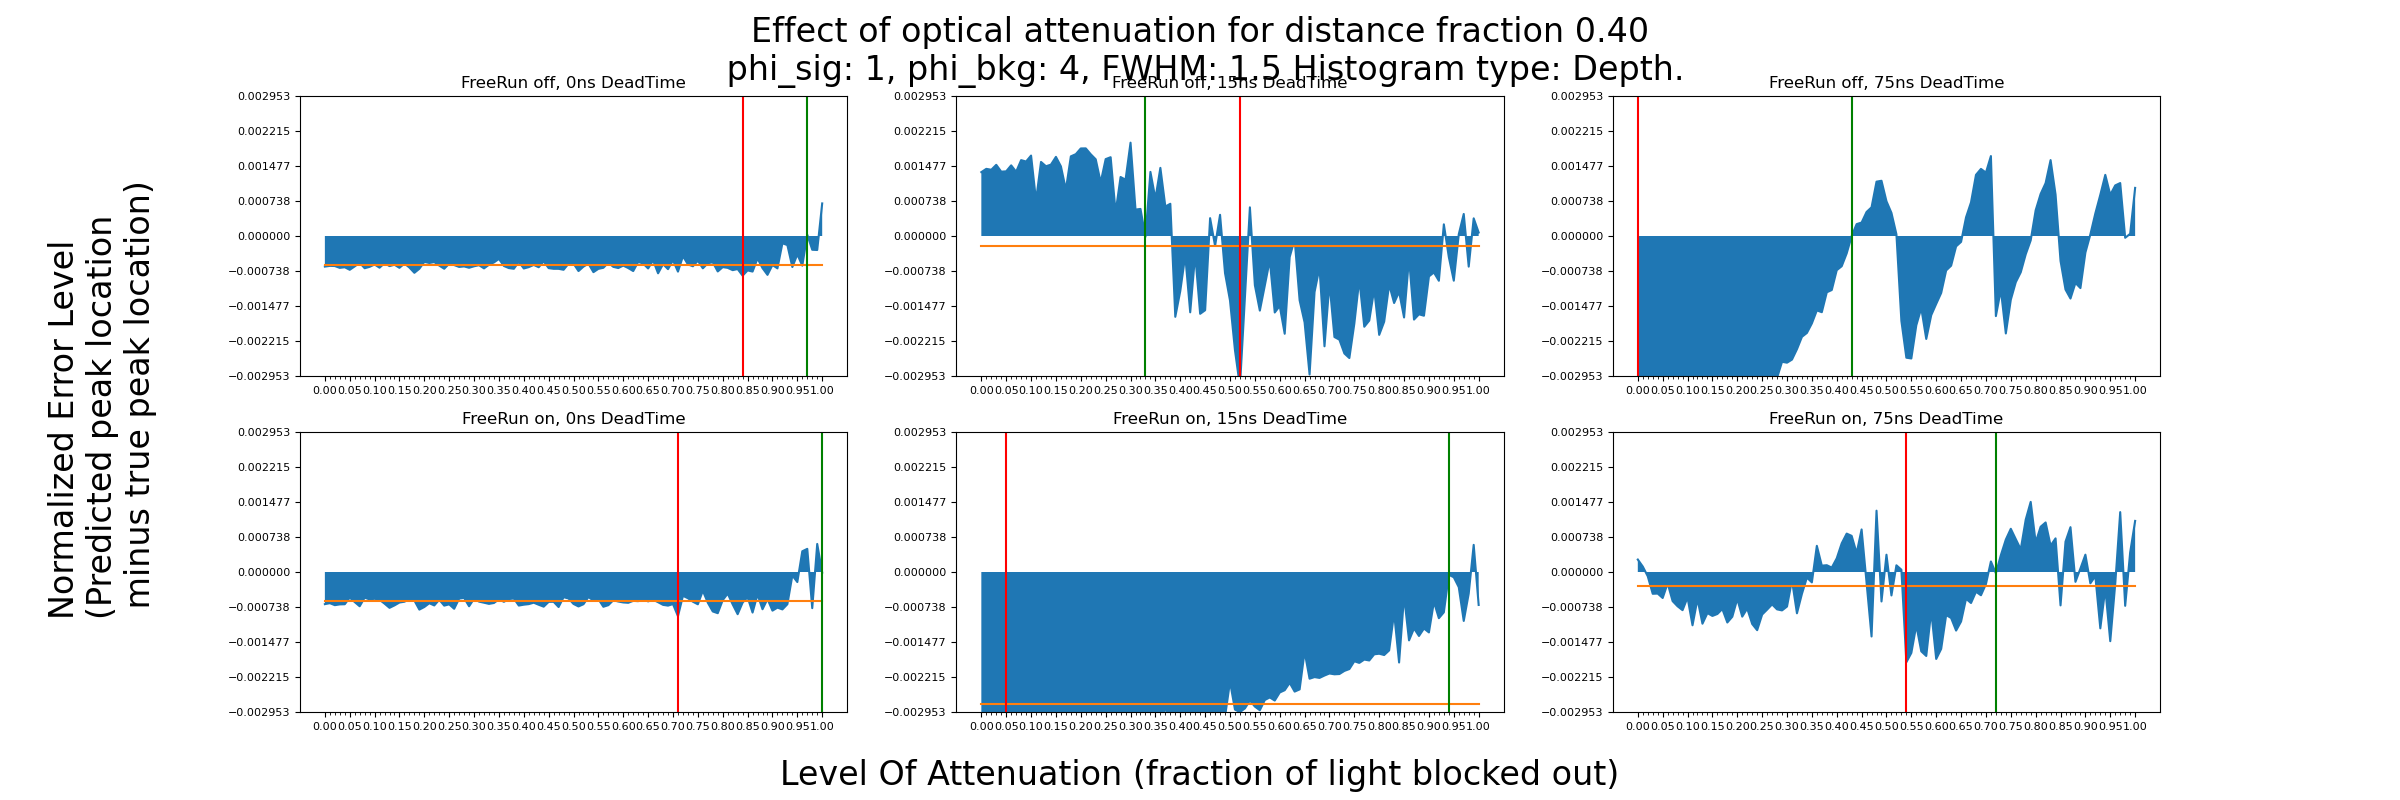
\includegraphics[width=1\linewidth]{sharedFreeExample.png}
\label{fig:sharedExample}
\end{subfigure}
\caption{\label{fig:freerunComparsion}Freerun and non-Freerun on different y axes.}
\end{figure}

\begin{figure}[H]
\centering
\begin{subfigure}[b]{1\textwidth}
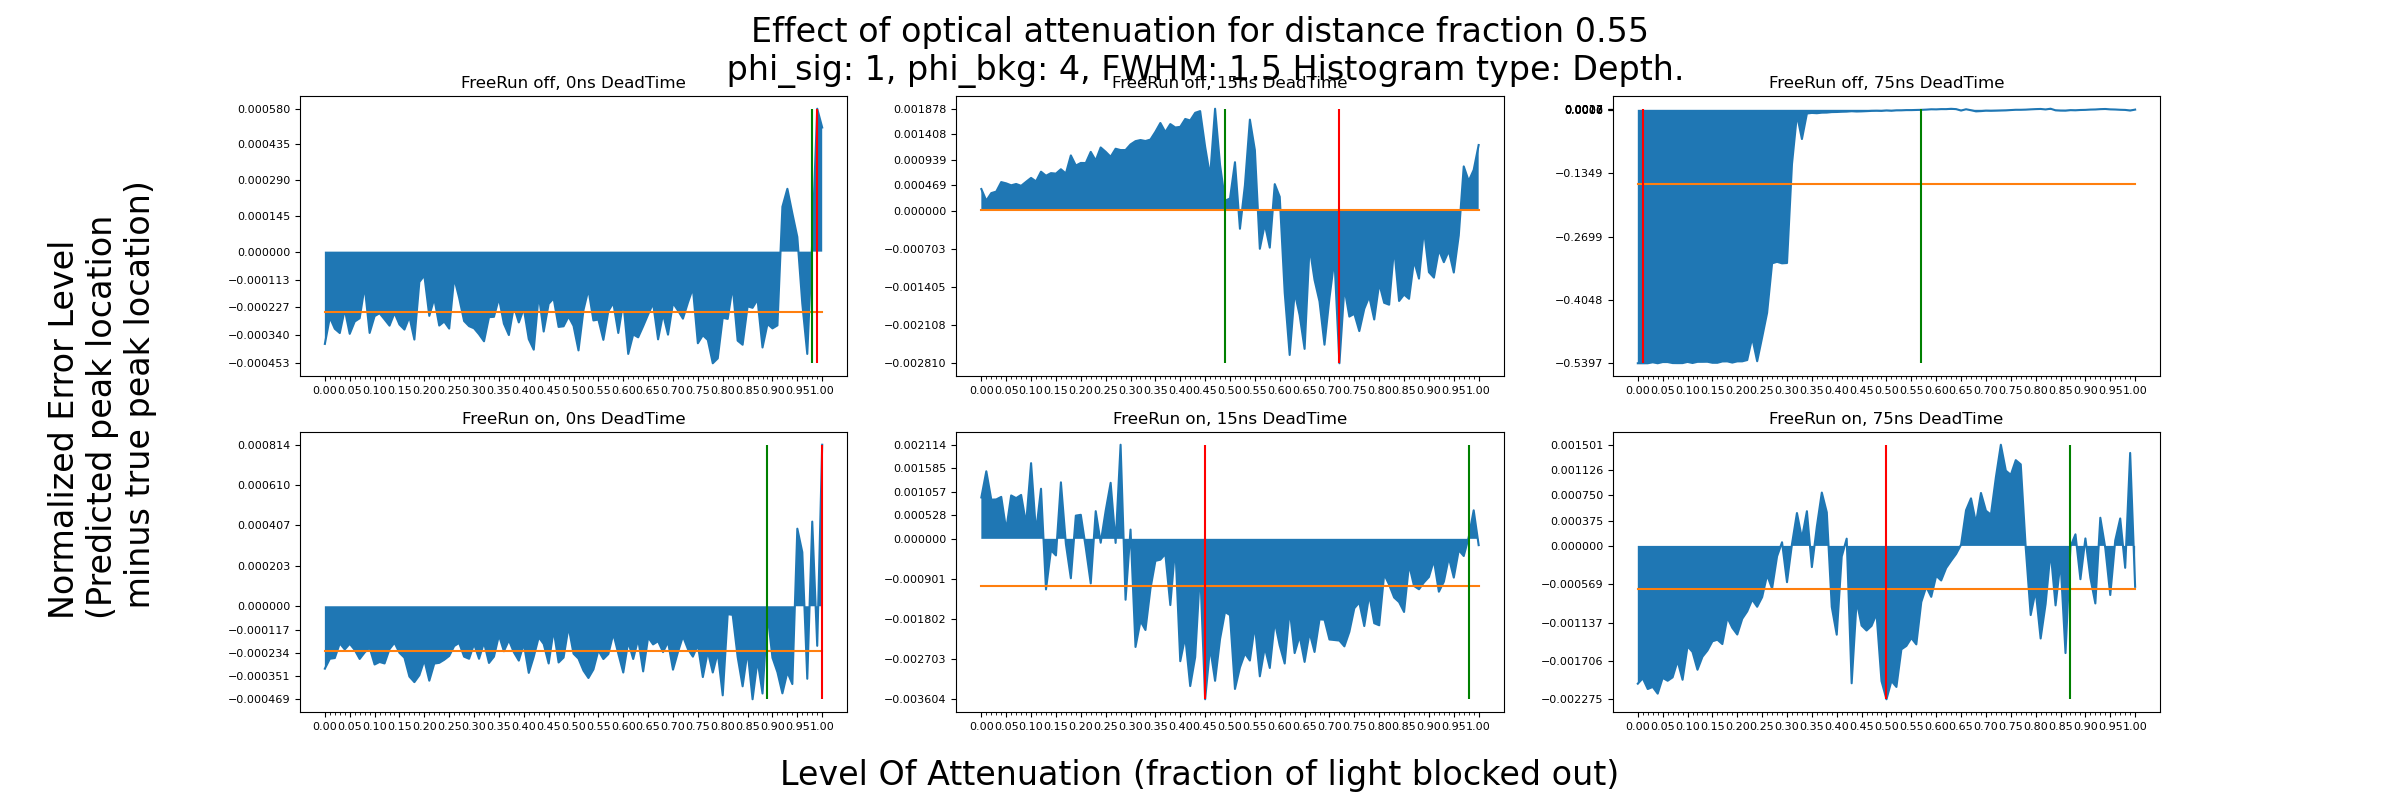
\includegraphics[width=1\linewidth]{1.5Example.png}
\label{fig:1.5Example}
\end{subfigure}
\begin{subfigure}[b]{1\textwidth}
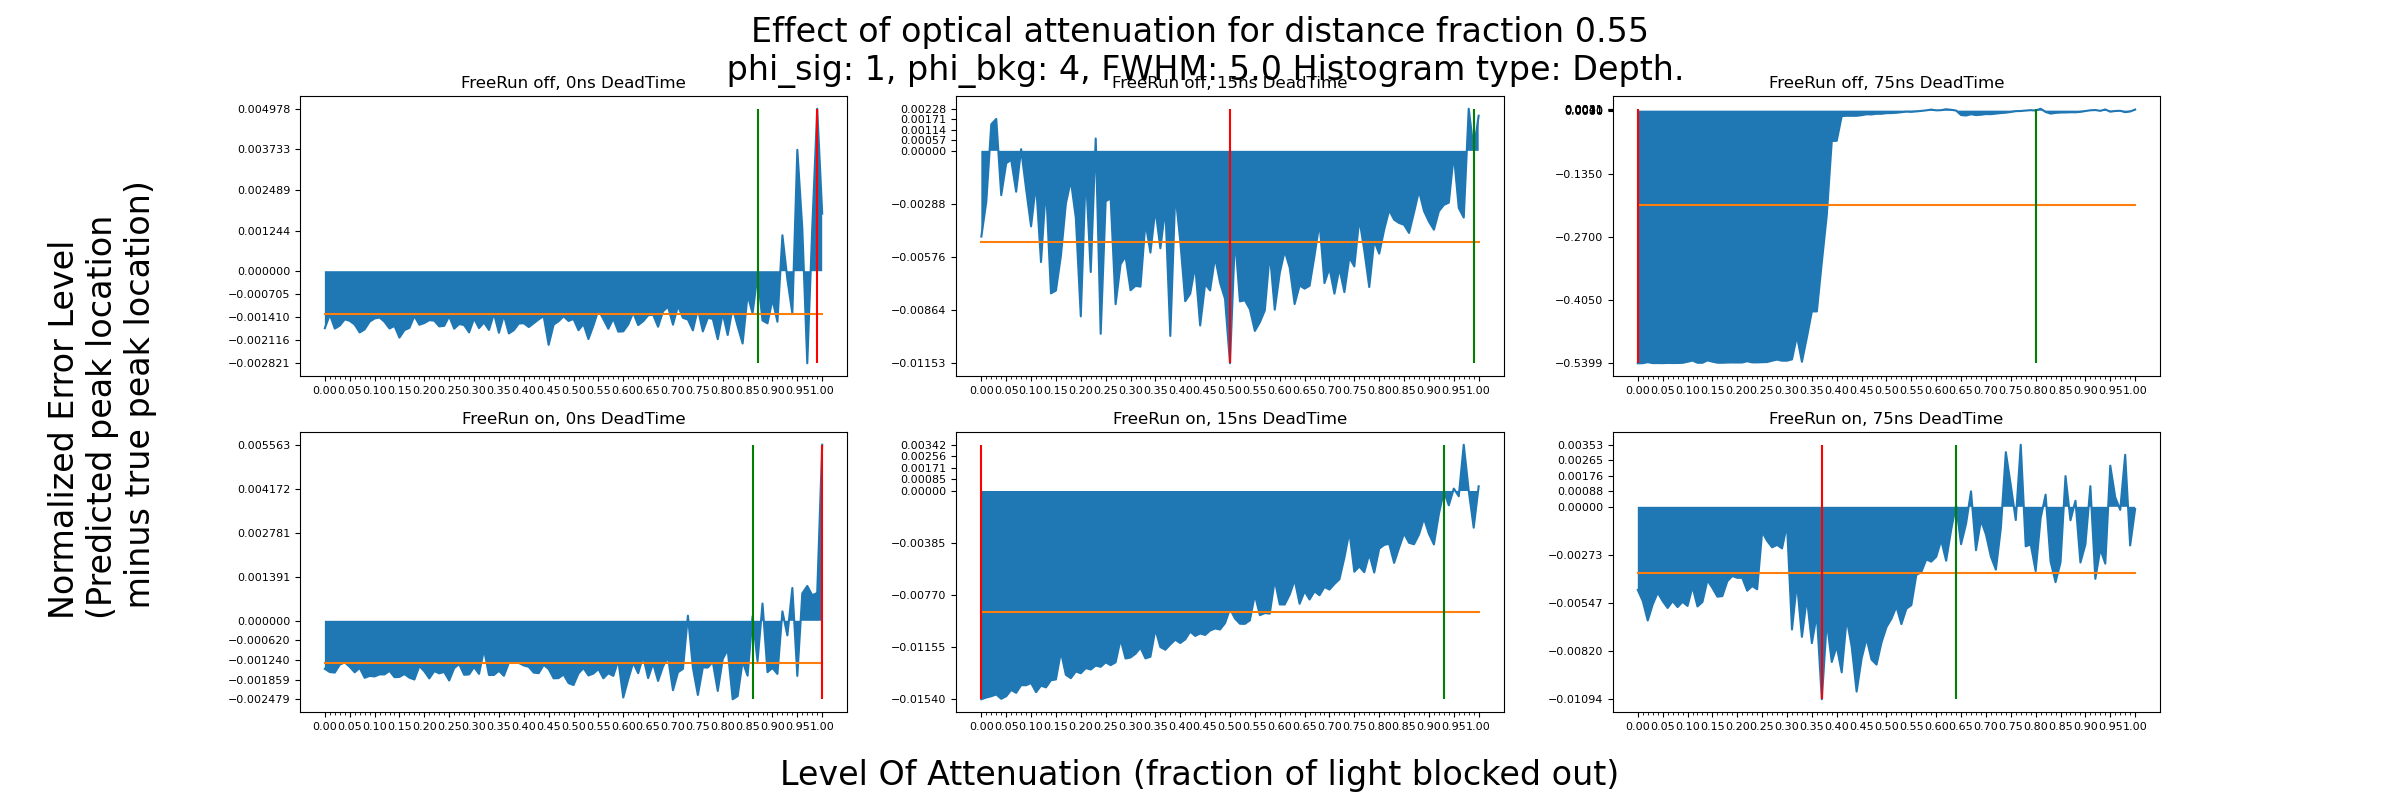
\includegraphics[width=1\linewidth]{5.0Example.png}
\label{fig:5.0Example}
\end{subfigure}
\caption{\label{fig:pulseComparison}1.5 FWHM vs 5.0 FWHM.}
\end{figure}

\section*{Discussion}
In Short, the results show that:
\begin{itemize}
  \item EDH Error Calculation with 16 buckets produces more error than EWH Error Calculation with 1000 buckets, which does not support our hypothesis that EDH Error Calculation with 16 buckets produces less error than EWH Error Calculation with 1000 buckets.
  \item FreeRun simulations produce less error than Non-Freerun simulations, which does support our hypothesis that FreeRun (asynchronous) simulations produce less error than Non-Freerun (parallel) simulations.
  \item 1.5 FWHM simulations produce less error than 5.0 FWHM simulations, which does not support our hypothesis that FreeRun simulations produce less error than Non-Freerun simulations.
\end{itemize}
While some of these results were different from our expectations, they are still explainable observations. Some possible explanations are as follows
\begin{itemize}
  \item EDH error calculation may require more than 16 buckets to match the accuraccy of EWH error calculation qith 1000 buckets.
  \item FreeRun simulations produce less skewed data, thus making their results more closely match reality.
  \item Higher FWHM simulations may produce wider peaks that that .
\end{itemize}
Our findings have a few implications for practial use of SPCs. The specific implications is that when trying to minimize error while taking SPC photographs...
\begin{itemize}
  \item One should use EWH error caclulation instead of EDH error calculation.
  \item One should use Asynchronous data collection (FreeRunning mode) instead of Parallel data collection.
  \item One should set their laser's FWHM to 1.5 instead of 5.0.
\end{itemize}

\section*{Limitations}
All data was collected using the SPCSimLib library, so any flaws in the methods by which it collects data would cause flaws in the data we have analyzed and graphed. Additionally, each simulation was prone to it's own fluctuations, and while we did take an average of 10 repeitions to reduce the error in our error measurements (meaning the difference between our average erorr measurements and base reality) there were still fluctuations in the data, despite the relatively clear trends.

\section*{Conclusion}
As Single Pixel Cameras develop and their use increases, it is important to know what settings will allow said SPCs to produce the most accurate pictures. After we repeatedly simulated  individual pixels of SPC cameras across several settings to collect enough data, we found that calculating error with EWH error calculation, Asynchronous Data Collection and 1.5 FWHM lasers produced the most accurate results. This implies that to produce highly-accurate pictures for SPC cameras, one should use said settings. From this, we propose that these become standard settings for SPC cameras, and suggest that more research be done into FWHM to figure out the optimal FWHM.

\printbibliography

\end{document}
